

%----------------------------------------------------------------------------------------
%	PACKAGES AND THEMES
%----------------------------------------------------------------------------------------


\documentclass{beamer}
\usetheme{Madrid}

\makeatletter
\setbeamertemplate{footline}
{
  \leavevmode%
  \hbox{%
  \begin{beamercolorbox}[wd=.3\paperwidth,ht=2.25ex,dp=1ex,center]{author in head/foot}%
    \usebeamerfont{Name in head/foot}\insertshortauthor
  \end{beamercolorbox}%
  \begin{beamercolorbox}[wd=.4\paperwidth,ht=2.25ex,dp=1ex,center]{title in head/foot}%
    \usebeamerfont{ Institute in head/foot}\insertshorttitle
  \end{beamercolorbox}%
  \begin{beamercolorbox}[wd=.3\paperwidth,ht=2.25ex,dp=1ex,right]{date in head/foot}%
    \usebeamerfont{date in head/foot}\insertshortdate{}\hspace*{2em}
    \insertframenumber{} / \inserttotalframenumber\hspace*{2ex} 
  \end{beamercolorbox}}%
  \vskip0pt%
}
\makeatother

%new command
%% Blackboard bold letters
\newcommand{\N}{\mathbb N}
\newcommand{\R}{\mathbb R}
\newcommand{\Q}{\mathbb Q}
\newcommand{\Z}{\mathbb Z}
\newcommand{\C}{\mathbb C}

%% Bold font letters
\newcommand{\bX}{\mathbf X}
\newcommand{\bY}{\mathbf Y}
\newcommand{\bA}{\mathbf A}
\newcommand{\bB}{\mathbf B}
\newcommand{\bM}{\mathbf M}
\newcommand{\bI}{\mathbf I}
\newcommand{\bU}{\mathbf U}
\newcommand{\bW}{\mathbf W}

\newcommand{\be}{\mathbf e}
%% bold Greek symbols
\newcommand{\balpha}{{\boldsymbol{\alpha}}}
\newcommand{\bbeta}{{\boldsymbol{\beta}}}
\newcommand{\bmu}{{\boldsymbol{\mu}}}
\newcommand{\bdeta}{{\boldsymbol{\eta}}}
\newcommand{\btheta}{{\boldsymbol{\theta}}}
\newcommand{\bseta}{\boldsymbol{\eta}}
\newcommand{\brho}{{\boldsymbol{\rho}}}
\newcommand{\bepsilon}{\boldsymbol{\epsilon}}
\newcommand{\bvarepsilon}{\boldsymbol{\varepsilon}}
\newcommand{\bgamma}{\boldsymbol{\gamma}}
\newcommand{\bomega}{{\boldsymbol{\omega}}}

\newcommand{\bOmega}{{\boldsymbol{\Omega}}}
\newcommand{\bSigma}{{\boldsymbol{\Sigma}}}
\newcommand{\bTheta}{{\boldsymbol{\Theta}}}

\DeclareMathOperator*{\argmax}{arg\,max}
\DeclareMathOperator*{\argmin}{arg\,min}
\newcommand{\Exp}{{\mathbb{E}}}
\newcommand{\ind}{{\mathbbm{1}}}
\newcommand{\RN}[1]{%
  \textup{\uppercase\expandafter{\romannumeral#1}}%
}

\usepackage{float}
\usepackage{caption}
\usepackage{subcaption}
\usepackage{cleveref}
\usepackage[round]{natbib}


\RequirePackage{amsmath}
\RequirePackage{amssymb}
\RequirePackage{amsthm}
\usepackage{amsfonts}
\usepackage{mathtools}
\usepackage{mathrsfs}

\usepackage{epsfig}
\usepackage{amscd}
\usepackage{graphicx}% Include figure files
\usepackage{dcolumn}% Align table columns on decimal point
\usepackage{bm}% bold math
\usepackage{enumerate}
\usepackage{tikz}
\usepackage{lineno,hyperref}
\usepackage{booktabs} % Allows the use of \toprule, \midrule and \bottomrule in tables

%----------------------------------------------------------------------------------------
%	TITLE PAGE
%----------------------------------------------------------------------------------------

\date{\today} % Date, can be changed to a custom date
\title[Department of Statistics and Operations Research]{Functional Sparse Estimation of Time Varying Graphical Model} % The short title appears at the bottom of every slide, the full title is only on the title page

\author[Meilei Jiang(UNC-CH)]{Meilei Jiang$^\text{\dag}$} % Your name
\institute % Your institution as it will appear on the bottom of every slide, may be shorthand to save space
{
$^\text{\dag}$Department of Statistics and Operations Research\\
 University of North Carolina at Chapel Hill \\ % Your institution for the title page
}


\begin{document}

\begin{frame}
\titlepage % Print the title page as the first slide
\end{frame}

\begin{frame}
\frametitle{Overview} % Table of contents slide, comment this block out to remove it
\tableofcontents % Throughout your presentation, if you choose to use \section{} and \subsection{} commands, these will automatically be printed on this slide as an overview of your presentation
\end{frame}


%\AtBeginSection[]
%{
%  \begin{frame}
%    \frametitle{Table of Contents}
%    \tableofcontents[currentsection]
 % \end{frame}
%}

\AtBeginSection[]
{
	\begin{frame}
		\frametitle{Outline}
		\tableofcontents[currentsection]
	\end{frame}
}

%----------------------------------------------------------------------------------------
%	PRESENTATION SLIDES
%----------------------------------------------------------------------------------------

%------------------------------------------------
\section{Introduction}

%------------------------------------------------
\begin{frame}
	\frametitle{Background}
	Precision matrix plays a fundamental role in many high dimensional inference problems.
	\begin{itemize}[<+->]
		\item Classification and discriminant analysis.
		\item Applications: portfolio optimization, speech recognition and genomics.
		\item Graphical Model: recovering the structure of undirected Gaussian graph is equivalent to the support of the precision matrix.
	\end{itemize}
	
\end{frame}

%------------------------------------------------
\begin{frame}
\frametitle{Gaussian Graphical Model}
\begin{itemize}[<+->]
\item $\bX = (X_1, \cdots, X_p) \sim \N(\mathbf{0}, \bSigma)$
    \begin{itemize}
    \item Precision matrix $\bOmega = \bSigma^{-1}$.
    \item Partial correlation between $X_j$ and $X_l$: $\rho^{jl} = -(\omega_{jl}/\sqrt{\omega_{jj}\omega_{ll}})$. 
    \end{itemize}
\item Graph $\mathcal{G} = (V, E)$ (Lauritzen, 1996).
    \begin{itemize}
    \item $V = \{ 1, \cdots, p\}$ is the set of nodes.
    \item $E = \left\{ (j, l) | X_j \text{ is conditionally dependent with } X_l, \text{given } X_{V/\{j, l\}}\right\}$
    \item $e_{jl} \in E$ if and only if $\rho^{jl} \neq 0$
    \item $e_{jl} \in E$ if and only if $\omega_{jl} \neq 0$
    \end{itemize}    
\item Estimation of $\mathcal{G}$ is equivalent to recover the non-zero entry of the precision matrix $\bOmega$.   
\end{itemize}
\end{frame}




%------------------------------------------------
\section{Sparse Gaussian Graphical Model Estimation}

%------------------------------------------------

\begin{frame}
	\frametitle{Estimation of $\bOmega$}
	\begin{itemize}[<+->]
		\item A random sample $\bX^{(1)}, \cdots, \bX^{(n)}$ of $\bX$
		\item When $n > p$, a nature estimator of $\bOmega$: $\hat{\bOmega}_n = \hat{\bSigma}_n^{-1}$
		\begin{itemize}
			\item $\hat{\bSigma}_n$ is the sample covariance matrix
		\end{itemize}
		\item When $n < p$, the estimation of $\bOmega$ becomes much more challenging due to singularity of $\hat{\bSigma}_n$.
	\end{itemize}
	
\end{frame}

%------------------------------------------------
\subsection{Neighborhood Selection Approach}
%------------------------------------------------
\begin{frame}
	\frametitle{Neighborhood Selection And Linear Regression}
	\pause
	Connection between linear regression and prediction matrix $\bOmega$: For each $j \in \left\{1 , \cdots, n\right\}$
	\begin{equation}
	\label{eq:regress1}
	\bX_j = \bX_{-j} \bbeta_j + \bvarepsilon_j = \sum_{\substack{l \neq j}} \bX_l \beta_{jl} + \bvarepsilon_j
	\end{equation}
	\begin{itemize}[<+->]
		\item $\beta_{jl} = \omega_{jl}/\omega_{jj}$
		\item The support of $\bbeta_j = \left\{\beta_{jl}; l \neq j \right\}$ (non-zero entries) is the neighborhood of node $j$. 
		\item Select the non-zero entry for $j$th row of $\bOmega$ is equivalent to the multivariate regression problem (\ref{eq:regress1}).     
	\end{itemize}
	
\end{frame}

%------------------------------------------------

\begin{frame}
	\frametitle{Neighborhood Selection Approach}
	
	\begin{itemize}[<+->]
		\item Meinshausen and B{\"u}hlmann (2006) applied Lasso least square regression on model (\ref{eq:regress1}) to estimate the support of $\bOmega$ row by row.
		\item Peng et al. (2012) considered a joint sparse regression to estimate the $p$ rows of $\bOmega$ together.
		\item Yuan (2010) applied Danzig selector on the multivariate regression problem (\ref{eq:regress1}) and estimated the entries of $\bOmega$ directly.   
		\item Graph structures can be recovered consistently in a high dimension settings. ( Meinshausen and B{\"u}hlmann, 2006; Peng et al, 2012) 
	\end{itemize}
	
\end{frame}



%------------------------------------------------
\subsection{Penalized Likelihood Estimation Approach}
%------------------------------------------------
\begin{frame}
\frametitle{Log-likelihood Estimation}
Another nature way is to estimate $\bOmega$ is the penalized likelihood approach.
\begin{itemize}[<+->]
\item Log-likelihood function: $l(\bX^(i), 1 \leq i \leq n|\bOmega) = -\text{tr}(\bOmega \hat{\bSigma}_n) + \log|\bOmega|$
\item Penalized likelihood estimator:
\begin{equation}
\label{eq:penalizedlikelihood}
\hat{\bOmega}_L = \arg\min \text{tr}(\bOmega \hat{\bSigma}_n) - \log|\bOmega| + \sum_{\substack{j\neq l}}\lambda_{jl} p_{jl}(|\omega_{jl}|)
\end{equation}   
\begin{itemize}
	\item Yuan and Lin (2007), Banerjee et al. (2008), Friedman et al. (2008), Rothman et al. (2008) studied the Lasso type estimator .
	\item Friedman et al. (2008) proposed a fast algorithm, \emph{glasso}, for Lasso type estimator. 
	\item Yuan and Lin (2007) studied the non-negative garrote estimator.
	\item Fan et al. (2009), Lam et al. (2009) studied the penalized likelihood estimator with the smoothly clipped absolute deviation (SCAD) penalty and the adaptive Lasso penalty.
\end{itemize}
\end{itemize}

\end{frame}



%------------------------------------------------
\subsection{Constrained $\ell_1$ Minimization Approach}
%------------------------------------------------

\begin{frame}
	\frametitle{Constrained $\ell_1$ Minimization Approach}
	\begin{itemize}[<+->]
		\item Cai et al. (2011) performed a constrained l1 minimization approach to estimate sparse precision matrix (CLIME).
		\begin{equation}
			\label{eq:clime}
			\begin{aligned}
			\hat{\bOmega}_1 &= \arg\min \|\bOmega\|_1, \text{subject to:} \\
			& |\bSigma_n^* \bOmega - \bI|_{\infty} \leq \tau_{n} \\
			\end{aligned}
		\end{equation}
        \item Problem~\ref{eq:clime} can be decomposed to $p$ vector-minimization problem:
        $$\hat{\bomega}_j = \arg\min |\bomega_j|_1 \text{ subject to} |\bSigma_n^* \bomega_j - \be_j|_{\infty} \leq \tau_{n}, 1 \leq j \leq p.$$
        \item Cai et al. (2016) proposed adaptive constrained l1 minimization estimator (ACLIME), which achieved the optimal minimax rate of convergence.
	\end{itemize}
\end{frame}

%------------------------------------------------
\section{Heterogeneous Data And Joint Estimation Of Multiple Graphs}

\begin{frame}

\frametitle{Joint Estimation of Multiple Graphical Models}

\begin{itemize}[<+->]
\item Data are heterogeneous with $p$ variables and $G$ groups.
    \begin{itemize}
    \item $\mathbf{X}_i^{(g)} = (X_{i,1}^{(g)}, X_{i,2}^{(g)}, \cdots, X_{i,p}^{(g)}) \sim \mathcal{N}(0, \bSigma^{(g)}), i = 1, \dots, n_g; g = 1, \dots, G.$
    \item $\left\{\bOmega \right\} = \left\{ \bOmega^{(g)} = (\bSigma^{(g)})^{-1}| g = 1 \cdots G \right\}$
    \end{itemize} 
       
\end{itemize}

\end{frame}


\begin{frame}	
	\frametitle{Joint Estimation of Multiple Graphical Models}
	Joint penalized likelihood of multiple precision matrices  
	\begin{equation}
	\label{eq:multiplegraph}
	\left\{\hat{\bOmega} \right\} = \argmin_{\substack{\left\{\bOmega \right\}}} \sum_{g = 1}^{G} n_g \left[ \text{tr}(\bOmega^{(g)} \hat{\bSigma}^{{g}}) - \log|\bOmega^{(g)}| \right] + P(\left\{\bOmega \right\})
	\end{equation}
	\begin{itemize}[<+->]
		\item  Guo et al. (2011) employs a non-convex penalty called \emph{hierarchical group penalty}: $P(\left\{\bOmega \right\}) = \lambda \sum_{\substack{j \neq l}}\left(\sum_{g = 1}^{G} |\omega_{jl}^{(g)}| \right)^{1/2}$
		\item Honorio and Samaras (2012) adopts a convex penalty, $P(\left\{\bOmega \right\}) = \lambda \sum_{\substack{j \neq l}} |\omega_{jl}^{(1)}, \cdots, \omega_{jl}^{(G)}|_q$.
		\item Danaher et al. (2014) considered a \emph{fused lasso penalty}, $P(\left\{\bOmega \right\}) = \lambda_1 \sum_{\substack{j \neq l}}\sum_{g = 1}^{G}|\omega_{jl}^{(g)}| + \lambda_2 \sum_{\substack{g < g'}}\sum_{\substack{jl}}|\omega_{jl}^{(g)} - \omega_{jl}^{(g')}|$.
	\end{itemize}
\end{frame}	


\begin{frame}	
	\frametitle{Joint Estimation of Multiple Graphical Models}
	\begin{itemize}[<+->]
		\item Lee and Liu (2015) decomposed $\left\{\bOmega \right\}$ into the common structure $M = \frac{1}{G} \sum_{\substack{g}} \bOmega^{(g)}$ and the individual structure $R^{(g)} = \bOmega^{(g)} - M$, and applied constrained $\ell_1$ minimization to estimate the parameters.       
	\end{itemize}
\end{frame}	

%------------------------------------------------

\section{Time Varying Graphical Model}
\begin{frame}

\frametitle{Time Varying Graphical Model}

It is not unusual that the index of groups of samples have a order. A common situation is that the data are collected by time order.

\begin{itemize}
    \item $\bX(t) \sim \mathcal(0, \bSigma(t)), t = t_1, \dots, t_n.$ 
    \begin{itemize}
    	\item Denote $\bX^i = \bX(t_i), i = 1, \cdots, n$.
    \end{itemize}
    \item Dynamic graph: $G(t) = (V, E(t))$
    \begin{itemize}
    	\item $V = \left\{1,\cdots, p\right\}$.
    	\item $E(t) = \left\{ (j,l) \in V^2 : \text{Cov} \left[ X_j(t), X_l(t)| X_k(t), k \neq j,l \right] \neq 0, j \neq l \right\}.$
    \end{itemize}
\end{itemize}
\end{frame}


%------------------------------------------------

\begin{frame}

\frametitle{Time Varying Graphical Model: Penalized likelihood estimation}

 Zhou (2010) developed a nonparametric framework for estimating time varying graphical model by kernel smoothing and $\ell_1$ penalty. 
\begin{equation}
\label{eq:kernel_likelihood}
\begin{aligned}
\hat{\bOmega}(\tau) &= \arg\min_{\bOmega} \left\{ \text{tr}(\bOmega \hat{\bSigma}(\tau)) - \log|\bOmega| + \lambda\|\bSigma^{-}\|_1 \right\}\\
\text{where }& \hat{\bOmega}(\tau) = \sum_i \omega_i^{\tau} \bX^i (\bX^i)', \text{and }\omega_i^{\tau} = \frac{K_h(t_i - \tau)}{\sum_{i'} K_h(t_{i'}- \tau)} \\
\end{aligned}
\end{equation}

\end{frame}

%------------------------------------------------
\subsection{Varying Coefficient Model}
%-----------------------------------------------
\begin{frame}

\frametitle{Time Varying Graphical Model And Varying Coefficient Model}

\begin{itemize}
    \item Dynamic partial correlation coefficient $\rho_{jl}(t) = - \omega_{jl}(t) / \sqrt{\omega_{jj}(t) \omega_{ll}(t)} $
    \item Dynamic neighborhood selection:
    \begin{equation}
    \label{eq:varycoefmodel}
    X_j(t) = \bX_{-j}'(t) \bbeta_j(t) + \varepsilon_j(t) = \sum_{\substack{l\neq j}} X_l(t) \beta_{jl}(t) + \varepsilon_j(t).
    \end{equation}
    \begin{itemize}
    	\item Varying coefficient model (Hastie and Tibshirani, 1993)
    \end{itemize}
    \item Kolar et al. (2009, 2010); Kolar and Xing (2011) proposed a local linear regression approach with “kernel $\ell_1$” penalty to estimate the smoothly varying graph,
    \begin{equation}
    \label{eq:smoothgraph}
    \hat{\bbeta}_j(\tau) = \argmin_{\substack{\bbeta \in \R^{p-1}}} \sum_i(X_j^i - \sum_{\substack{l\neq j}} X_l^i \beta_l)^2 \omega_i^{\tau} + \lambda|\bbeta|_1
    \end{equation}
\end{itemize}

\end{frame}

%------------------------------------------------

\begin{frame}
\frametitle{Time Varying Graphical Model And Varying Coefficient Model}
\begin{itemize}
	\item Kolar et al. (2009, 2010); Kolar and Xing (2011, 2012) proposed a combination of $\ell_1$ and fused lasso penalty to estimate graph with jump.
	\begin{equation}
	\label{eq:jumpgraph}
	\begin{aligned}
	&\left\{ \hat{\bbeta}_j(t_1), \cdots, \hat{\bbeta}_j(t_n) \right\} =\\ &\argmin_{\substack{\bbeta(t_i), i \leq n}} \sum_i(X_j^i - \sum_{\substack{l\neq j}} X_l^i \beta_l(t_i))^2  + \lambda_1 \sum_{i}|\bbeta(t_i)|_1 \\
	&+ \lambda_2 \sum_{i = 2}^n|\bbeta(t_i) - \bbeta(t_{i-1})|_1
	\end{aligned}	
	\end{equation}
\end{itemize}

\end{frame}

%------------------------------------------------

\begin{frame}
	\frametitle{Time Varying Graphical Model And Functional Coefficient Model: Motivation}

Limitation of aforementioned method:
\pause
\begin{itemize}[<+->]
	\item Apply local linear regression on the model (\ref{eq:smoothgraph}) can only get the estimation on input time point.
	\item The assumption in the model (\ref{eq:jumpgraph}) of the coefficient is piecewise constant is usually not realistic.
\end{itemize}
Use basis expansion to estimate $\bbeta_j(t)$ directly.
	
\end{frame}

%------------------------------------------------
\subsection{Functional Coefficient Model}
%------------------------------------------------
\begin{frame}
	\frametitle{Functional Coefficient Model}
	\begin{itemize}[<+->]
		\item Assuming data are collected at $t_1, \cdots, t_n$, and at each time point $t$, we have $n_t$ replicates (Huang et al, 2004). 
		\begin{equation} 
		\label{eq:flm}
		\begin{aligned}
		X_j^r(t) &= {\bX_{-j}^r(t)}' \bbeta_j(t) + \varepsilon_j^r(t)\\
		&= \sum_{\substack{l\neq j}} X_l^r(t) \beta_{jl}(t) + \varepsilon_j^r(t),\\
		\end{aligned} 
		\end{equation}
		\begin{itemize}
			\item $\bX_{-j}^r(t) = (X_l^r(t))_{\substack{l \neq j}} \in \R^{(p-1) \times 1}, r = 1, \cdots, n_t$.
			\item $t = t_1, \cdots, t_n, j = 1, \cdots, p$.
		\end{itemize}
		\item For each $t$, let $\bX_j(t) = (X_j^1(t), \cdots, X_j^{n_t}(t))^T \in \R^{n_t \times 1}$, then 
		\begin{equation}
			\label{eq:flm0}
			\begin{aligned}
			\bX_j(t) &= {\bX_{-j}(t)}' \bbeta_j(t) + \bvarepsilon_j(t)\\
			&= \sum_{\substack{l\neq j}} \bX_l(t) \beta_{jl}(t) + \bvarepsilon_j(t),\\
			\end{aligned}
		\end{equation}
	\end{itemize}
	
	
	
\end{frame}

%------------------------------------------------

\begin{frame}
	\frametitle{Functional Coefficient Model}
	\begin{itemize}
		\item For each functional coefficient $\beta_{jl}(t)$, we consider the basis expansion $\bB_{jl}(t) = (B_{jl1}(t), \cdots, B_{jlk_{jl}}(t) )$: 
		$$\beta_{jl}(t) = \sum_{\substack{s=1}}^{k_{jl}} B_{jls}(t) \gamma_{jls} + e_{jl}(t) = \bB_{jl}(t) \bgamma_{jl} + e_{jl}(t)$$
		\item $\bbeta_j(t) = \bB(t) \bgamma_j + \be_j(t) = (\beta_{jl}|j \neq l) \in \R^{p-1}$
		\begin{itemize}
			\item $\bB(t) = \text{diag}\left\{\bB_{jl}(t)\right\} \in \R^{(p-1)\times \sum_{\substack{l \neq j}}k_{jl} }$
			\item $\bgamma_j = (\bgamma_{jl})_{l \neq j} \in \R^{\sum_{\substack{l \neq j}}k_{jl} \times 1}$
			\item $\be(t) = (\be_{jl}|j \neq l) \in \R^{p-1}$
		\end{itemize}
	\end{itemize}
	
\end{frame}	
%------------------------------------------------

\begin{frame}
	\frametitle{Functional Coefficient Model}
	\pause
	Thus Equation~(\ref{eq:flm}) can be represented as
	\pause
	\begin{equation}
	\label{eq:flm2}
	\begin{aligned}
	\bX_j(t) &= \bX_{-j}(t) \bB_j(t) \bgamma_j + \tilde{\bvarepsilon}(t) \\
	&= \bU(t) \bgamma_j + \tilde{\bvarepsilon}(t),\\
	\text{where } \bU(t) &= \bX_{-j}(t) \bB_j(t)\in \R^{\sum_{t = 1}^{n}n_t \times \sum_{\substack{j \neq i}}k_{jl}},\\
	\tilde{\bvarepsilon}(t) &= \bX_{-j}(t)\be_j(t) + \bvarepsilon(t)\\
	&= \sum_{\substack{l \neq j}} \bX_l(t)e_{jl}(t) + \bvarepsilon(t),\\
	t &= t_1, \cdots, t_n, j = 1, \cdots, p.\\
	\end{aligned}
	\end{equation}
	\pause
	As seen in Equation~(\ref{eq:flm2}), our model is quite flexible since the basis of each functional coefficient can be different.
\end{frame}	
%------------------------------------------------

\begin{frame}
	\frametitle{Functional Coefficient Model}
	Combing the data from $t_1, \cdots, t_n$, we can get
	\begin{equation}
	\label{eq:flm3}
	\begin{aligned}
	\bX_j &= \bU_j \bgamma_j + \tilde{\bvarepsilon}_j, j = 1, \cdots, p.\\
	\text{where }\bX_j &= (X_j(t_1)', \cdots, X_j(t_n)')' \in \R^{\sum_{t = 1}^{n}n_t \times 1}\\
	\bU_j &= ( \bU_j(t_1)', \cdots, \bU_j(t_n)' )' \in \R^{\sum_{t = 1}^{n}n_t \times \sum_{\substack{j \neq i}}k_{jl}}\\
	\tilde{\bvarepsilon}_j &= (\tilde{\bvarepsilon}_j(t_1), \cdots, \tilde{\bvarepsilon}_j(t_n))^T \in \R^{\sum_{t = 1}^{n}n_t \times 1}
	\end{aligned}	
	\end{equation}
	For each $j$, least square of $\bgamma_j$ in the model~\ref{eq:flm3} is
	$$\begin{aligned}
	l(\bgamma_j) &= (\bX_j - \bU_j \bgamma_j)'\bW (\bX_j - \bU_j \bgamma_j)\\
	&= \sum_{i = 1}^{n}(\bX_j(t_i) - \bU_j(t_i) \bgamma_j)^2 w_i\\
	&= \sum_{i = 1}^{n}(\bX_j(t_i) - \bX_{-j}(t_i) \bbeta_j(t_i))^2 w_i\\
	\end{aligned}$$
\end{frame}	
%------------------------------------------------

\begin{frame}
	\frametitle{Functional Coefficient Model: Control Derivatives Sparsity}
   In Model~(\ref{eq:flm3}), we want to estimate a sparse graph and interpretable coefficient functions. 
   \pause
   \begin{itemize}[<+->]
   	\item For each $j$ and $l \neq j$, put $\ell_1$ penalty on $ \beta_{jl}^{(m)} = \frac{\mathrm{d^m}}{\mathrm{d} t^m} \beta_{jl}(t) \approx \frac{\mathrm{d^m}}{\mathrm{d} t^m} \bB_{jl}(t) \bgamma_{jl}$ for some $m$.
   	\item Assume $\beta_{jl}^{(0)}(t) = 0$ and $\beta_{jl}^{(2)}(t) = 0$ in large area, then $\beta_{jl}(t)$ is zero in many region and linear in the left regions.
   	\item Let $\bA^{(m)}(t) = \frac{\mathrm{d^m}}{\mathrm{d} t^m} \bB(t) \in \R^{(p-1)\times \sum_{\substack{l \neq j}}k_{jl} }$ and $\bA^{(m)} = (\bA^{(m)}(t_1)', \cdots, \bA^{(m)}(t_n)')' \in \R^{n(p-1)\times \sum_{\substack{l \neq j}}k_{jl} }$
   \end{itemize}
   \pause
   The penalty for Model~(\ref{eq:flm3}) is
   $$\begin{aligned}
   p(\bgamma_j) &= \lambda_0|\bA^{(0)} \bgamma_j|_1 + \lambda_m |\bA^{(m)} \bgamma_j|_1\\
   &= \sum_{i=1}^{n}\lambda_0|\bbeta_j^{(0)}(t_i)|_1 + \sum_{i=1}^{n}\lambda_2|\bbeta_j^{(m)}(t_i)|_1
   \end{aligned}$$   
	
\end{frame}	

%------------------------------------------------

\begin{frame}
	\frametitle{Functional Coefficient Model: Optimization Problem}
	The optimization problem for Model~(\ref{eq:flm3}) with sparse coefficient derivatives:
	\begin{equation}
	    \label{eq:opt}
	    \begin{aligned}
	    \mathcal{J}(\bgamma_j) &= l(\bgamma_j) + p (\bgamma_j)\\
	    &= (\bX_j - \bU_j \bgamma_j)'\bW (\bX_j - \bU_j \bgamma_j) + \lambda_0|\bA^{(0)} \bgamma_j|_1 + \lambda_m |\bA^{(m)} \bgamma_j|_1 \\
	    &= \sum_{i = 1}^{n}(\bX_j(t_i) - \bX_{-j}(t_i) \bbeta_j(t_i))^2 w_i +\\ &\sum_{i=1}^{n}\lambda_0|\bbeta_j^{(0)}(t_i)|_1 + \sum_{i=1}^{n}\lambda_m|\bbeta_j^{(m)}(t_i)|_1\\
	    \end{aligned}
	\end{equation}
	This is a generalized lasso optimization problem (Tibshirani, 2011).
\end{frame}	

%------------------------------------------------
\section{Simulation Study}
%------------------------------------------------
\begin{frame}
	\frametitle{Simulation}
	\begin{figure}
		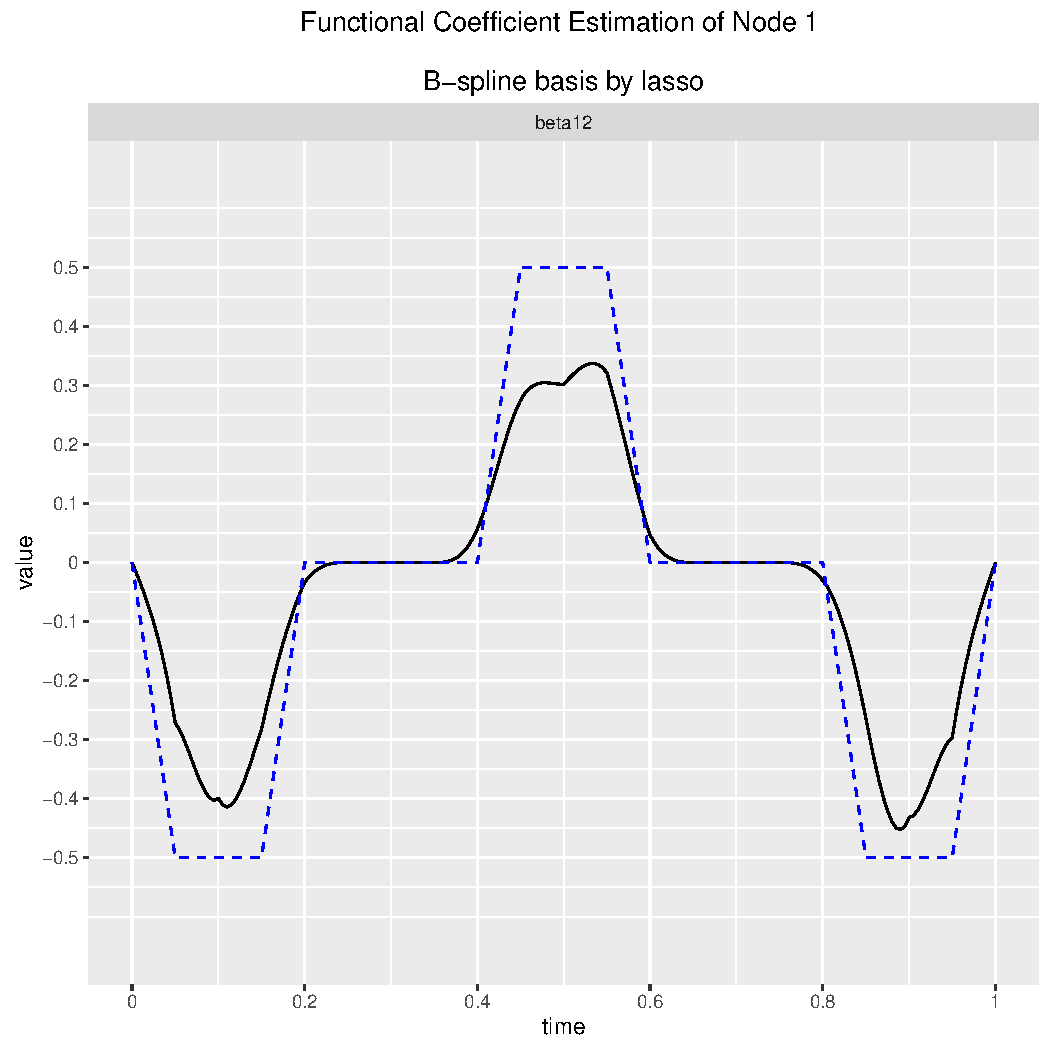
\includegraphics[height = 6cm]{2dexample_lasso.pdf}
	\end{figure}
\end{frame}
\begin{frame}
	\frametitle{Simulation}
	\begin{figure}
		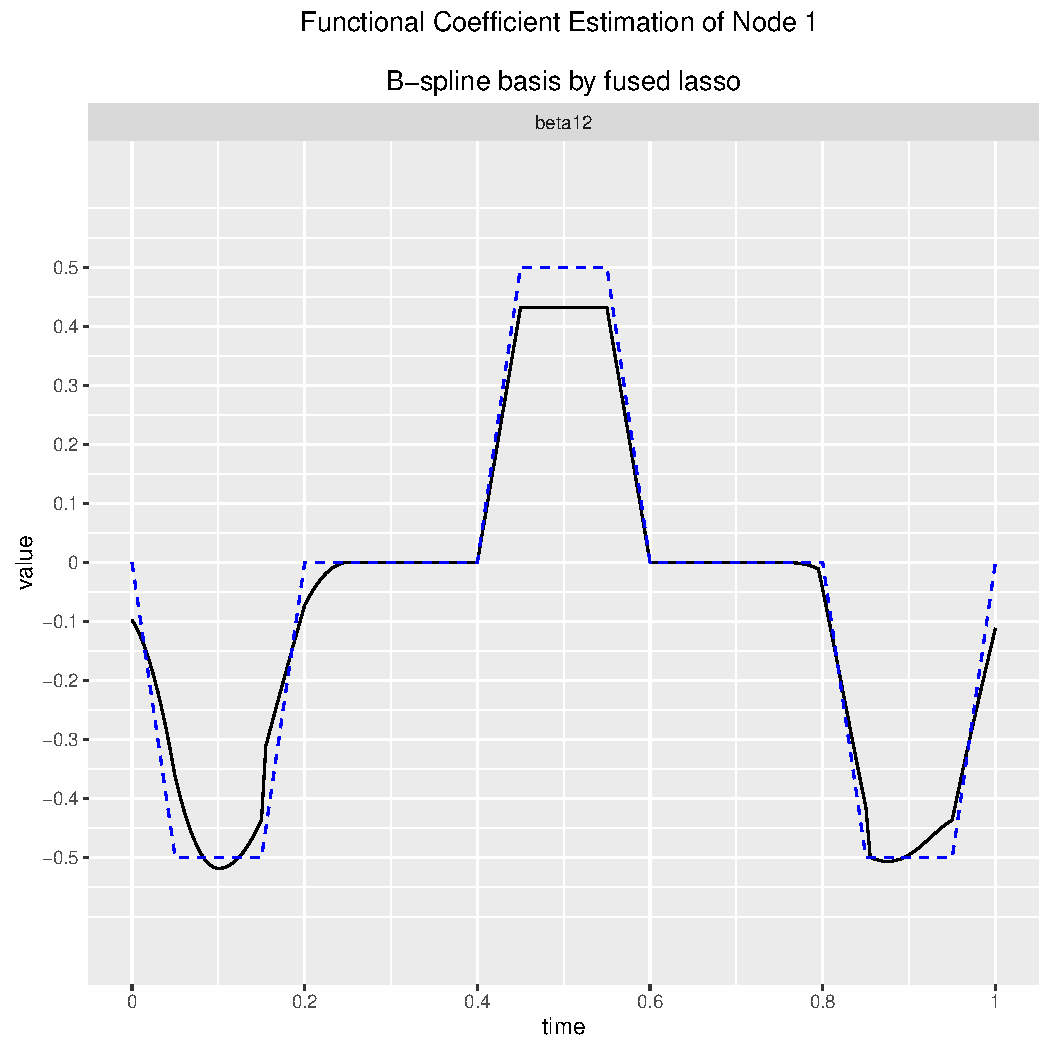
\includegraphics[height = 6cm]{2dexample_fused_lasso.pdf}
	\end{figure}
\end{frame}

\begin{frame}
	\frametitle{Simulation}
	\begin{figure}
		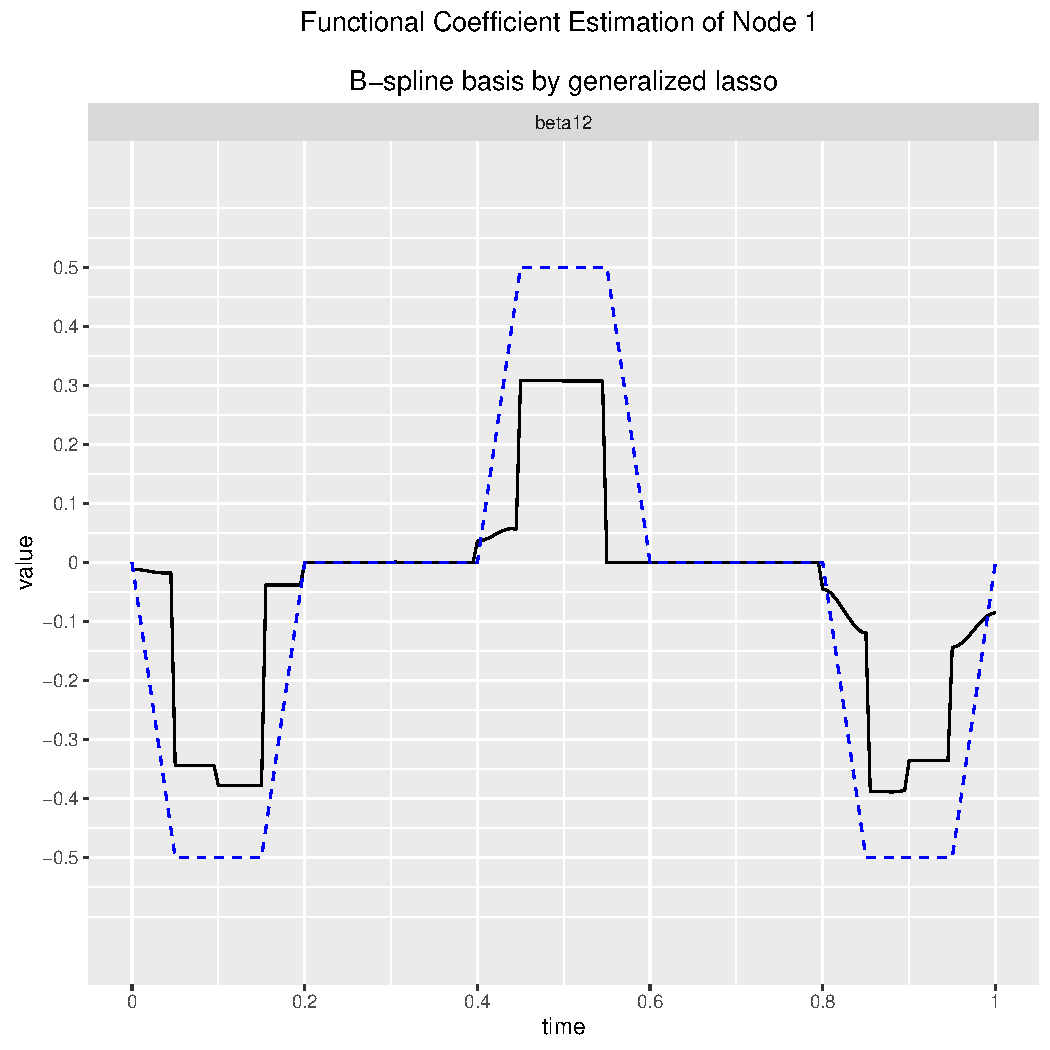
\includegraphics[height = 6cm]{2dexample_genlasso.pdf}
	\end{figure}
\end{frame}

%------------------------------------------------
\end{document}